\begin{figure}[H]
\centering

\begin{subfigure}{0.45\textwidth}
  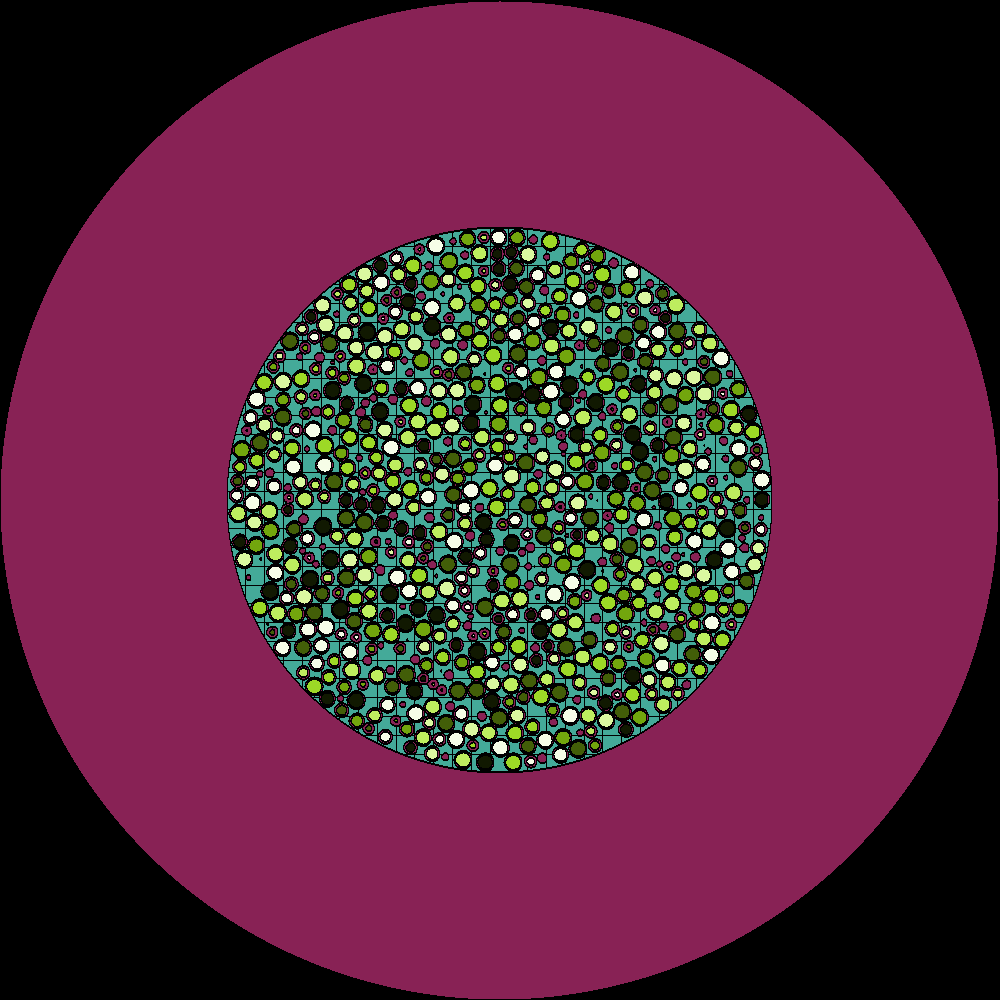
\includegraphics[width=0.95\linewidth]{figures/control/control-r}
  \caption{Radial Cross Section at y=0}
  \label{fig:controla}
\end{subfigure}%
%
\begin{subfigure}{0.45\textwidth}
  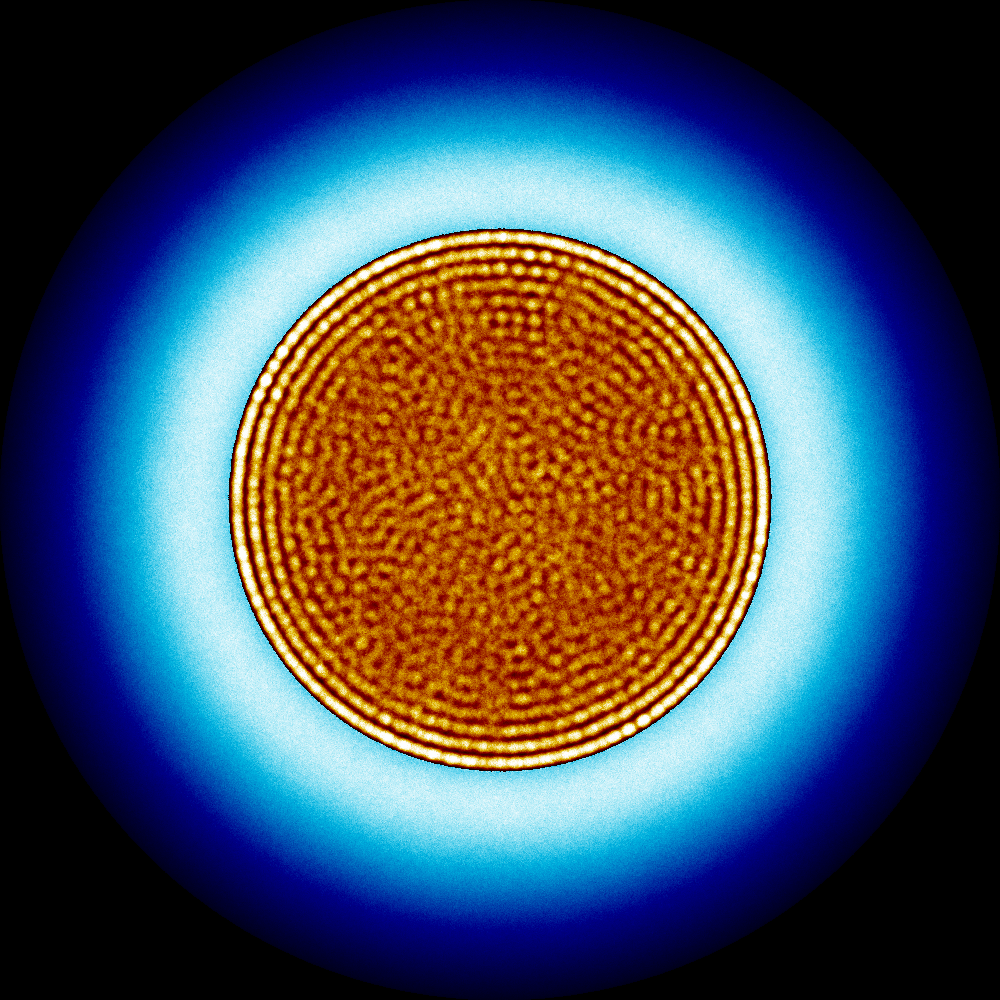
\includegraphics[width=0.95\linewidth]{figures/control/control-rm}
  \caption{Radial Mesh}
  \label{fig:controlb}
\end{subfigure}

\begin{subfigure}{0.45\textwidth}
  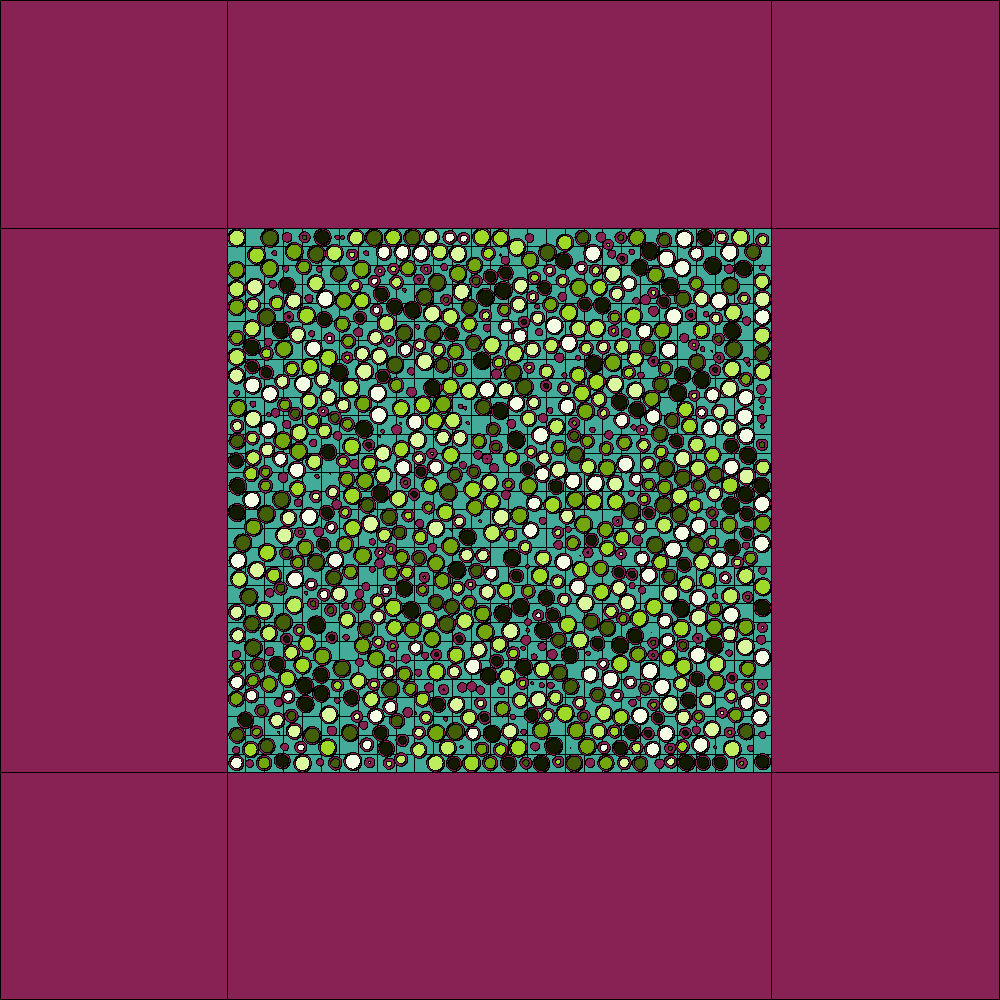
\includegraphics[width=0.95\linewidth]{figures/control/control-v}
  \caption{Axial Cross Section at z=0 }
  \label{fig:controlc}
\end{subfigure}
%
\begin{subfigure}{0.45\textwidth}
  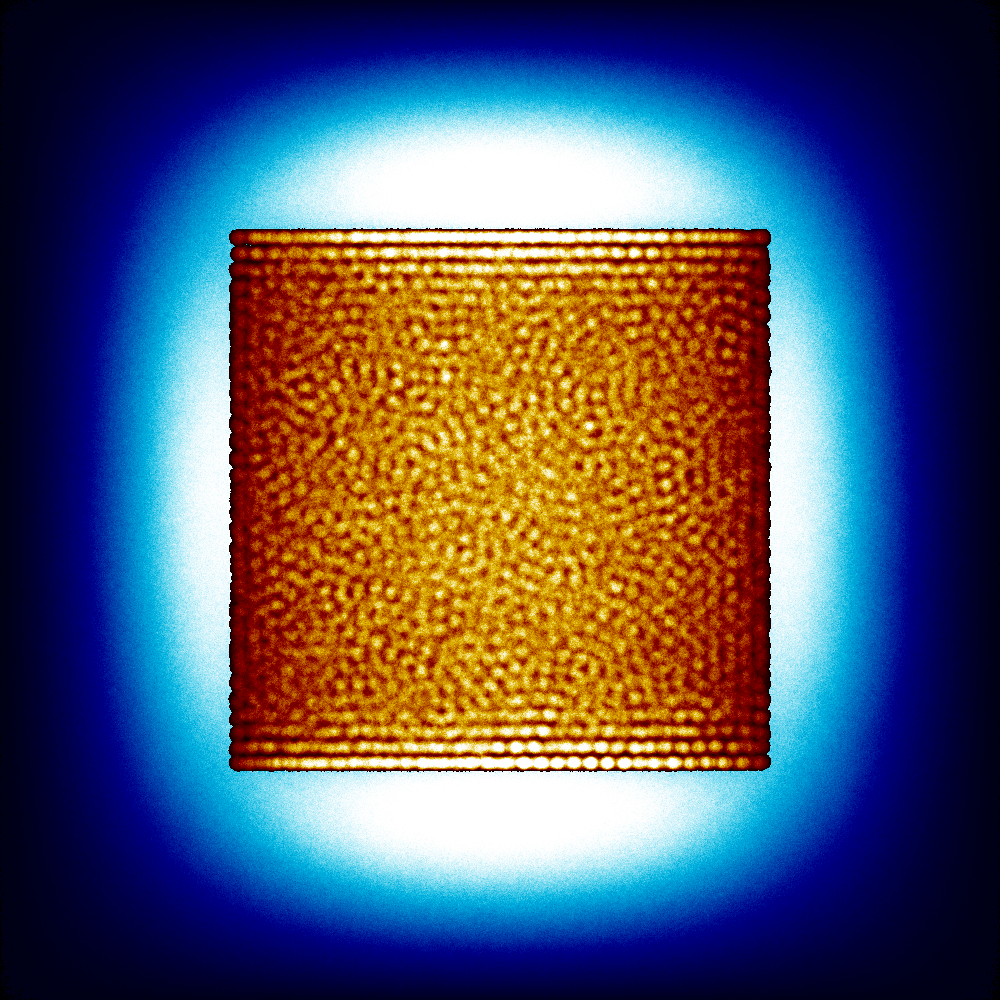
\includegraphics[width=0.95\linewidth]{figures/control/control-vm}
  \caption{Axial Mesh}
  \label{fig:controld}
\end{subfigure}
%
\begin{subfigure}{\textwidth}
\centering
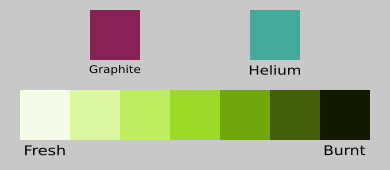
\includegraphics[width=0.6\linewidth]{figures/geom-legend}
\caption{Legend for \ref{fig:controla} and \ref{fig:controlc}}
\label{fig:geom-legend1}
\end{subfigure}

\caption{Geometry Cross Sections (left) and Thermal Flux(cold color map) and Fission Rate (hot color map) Meshes (right) for the Control Model of Sangamon20}
\label{fig:controlmain}
\end{figure}